\documentclass[journal,12pt,onecolumn]{IEEEtran}
\usepackage{amsmath,amsfonts}
\usepackage{amssymb}
\usepackage[utf8]{inputenc}
\usepackage{gensymb}
\usepackage{mathtools}
\usepackage{listings}
\begin{document}
\centering \textbf{Local Server On Raspberry Pi}\\
\begin{flushleft}
\textbf{Introduction:}  The Raspberry Pi can be used as a wireless access point, running a standalone network. This can be done using the inbuilt wireless features of the Raspberry Pi 3 or Raspberry Pi Zero, or by using a suitable USB wireless dongle that supports access points.\\
\medskip
In this Manual we will set up the Raspberry Pi as Standalone Network and using Apache2 we will create a local server to access the file.\\
\medskip

\textbf{Note:} \textit{This documentation was tested on a Raspberry Pi 3, and it is possible that some USB dongles may need slight changes to their settings.}\\
\medskip
In order to work as an access point, the Raspberry Pi will need to have access point software installed, along with DHCP server software to provide connecting devices with a network address. Ensure that your Raspberry Pi is using an up-to-date version of Raspbian (dated 2017 or later).\\ 
\bigskip
\textbf{Installation and Updates:}\\
\bigskip
$\bullet$  First of all you need to connect your Raspberry PI with normal monitor to install some required software.\\
\bigskip
$\bullet$  Raspberry PI should have a internet connection.\\
\bigskip
$\bullet$  Now run the following two commands one by one given below. \\ 
\bigskip
\begin{lstlisting}[frame=single,linewidth=7cm,breaklines=true]
sudo apt-get update
sudo apt-get upgrade

\end{lstlisting}
\bigskip

$\bullet$ Now you need to install \textbf{Hostapd} (Host access point daemon) is a user space software access point capable of turning normal network interface cards into access points and authentication servers.\\
other one is\\
\medskip
\textbf{Dnsmasq:} It provides Domain Name System (DNS) forwarder, Dynamic Host Configuration Protocol (DHCP) server, router advertisement and network boot features for small computer networks, created as free software.\\
\medskip
$\bullet$ Install the softwares in one go with this command:\\
\bigskip
\begin{lstlisting}[frame=single,linewidth=10cm,breaklines=true]
sudo apt-get install dnsmasq hostapd
\end{lstlisting}
\bigskip
$\bullet$ Since the configuration files are not ready yet, turn off the new software as follows:\\
\medskip
\begin{lstlisting}[frame=single,linewidth=8cm,breaklines=true]
sudo systemctl stop dnsmasq
sudo systemctl stop hostapd
\end{lstlisting}
\bigskip
$\bullet$ To ensure that an updated kernel is configured correctly after install, reboot:\\
\medskip
\begin{lstlisting}[frame=single,linewidth=5cm,breaklines=true]
sudo reboot
\end{lstlisting}
\bigskip

\textbf{Configuring a static IP:} \\
\bigskip
We are configuring a standalone network to act as a server, so the Raspberry Pi needs to have a static IP address assigned to the wireless port. This documentation assumes that we are using the standard 192.168.x.x IP addresses for our wireless network, so we will assign the server the IP address 192.168.4.1. It is also assumed that the wireless device being used is wlan0. \\
\bigskip
$\bullet$ To configure the static IP address, edit the dhcpcd configuration file with: \\
\bigskip
\begin{lstlisting}[frame=single,linewidth=8cm,breaklines=true]
sudo nano /etc/dhcpcd.conf
\end{lstlisting}
\bigskip

$\bullet$ Go to the end of the file and edit it so that it looks like the following:\\
\bigskip
\begin{lstlisting}[frame=single,linewidth=10cm,breaklines=true]
interface wlan0
    static ip_address=192.168.4.1/24
    nohook wpa_supplicant
\end{lstlisting}
\bigskip

$\bullet$ Now restart the dhcpcd daemon and set up the new wlan0 configuration:\\
\bigskip
\begin{lstlisting}[frame=single,linewidth=8cm,breaklines=true]
sudo service dhcpcd restart
\end{lstlisting}
\bigskip

\textbf{Configuring the DHCP server (dnsmasq):} \\

The DHCP service is provided by dnsmasq. By default, the configuration file contains a lot of information that is not needed, and it is easier to start from scratch.\\ 
\medskip
$\bullet$ Rename this configuration file, and edit a new one: \\
\bigskip
\begin{lstlisting}[frame=single,linewidth=15cm,breaklines=true]
sudo mv /etc/dnsmasq.conf /etc/dnsmasq.conf.orig  
\end{lstlisting}
\bigskip

Now open the dnsmasq configuration file. \\
\bigskip
\begin{lstlisting}[frame=single,linewidth=15cm,breaklines=true]
sudo nano /etc/dnsmasq.conf 
\end{lstlisting}
\bigskip

Now type the following information into the dnsmasq configuration file and save it:\\
\bigskip
\begin{lstlisting}[frame=single,linewidth=15cm,breaklines=true]
interface=wlan0      # Use the require wireless interface - usually wlan0
  dhcp-range=192.168.4.2,192.168.4.20,255.255.255.0,24h
\end{lstlisting}
\bigskip

So for wlan0, we are going to provide IP addresses between 192.168.4.2 and 192.168.4.20, with a lease time of 24 hours. If you are providing DHCP services for other network devices (e.g. eth0), you could add more sections with the appropriate interface header, with the range of addresses you intend to provide to that interface. \\
\bigskip
\textbf{Configuring the access point host software (hostapd):} \\
\medskip

You need to edit the hostapd configuration file, located at \textbf{/etc/hostapd/hostapd.conf}, to add the various parameters for your wireless network. After initial install, this will be a new/empty file.\\
\medskip
\bigskip
\begin{lstlisting}[frame=single,linewidth=10cm,breaklines=true]
sudo nano /etc/hostapd/hostapd.conf
\end{lstlisting}
\bigskip
Add the information below to the configuration file. This configuration assumes we are using channel 7, with a network name(SSID): \textbf{"ncr"}, you can set any name on SSID and wpa\_passphrase(password for the same SSID): \textbf{"abc12345"}.\\
\medskip
\textbf {\textit{Note that the SSID name and passphrase (password) should not have quotes around them. Here quotes are just to notify. The wpa\_passphrase should be between 8 to 64 characters in length and alphanumeric.}}
\bigskip
Add these following lines to \textbf{/etc/hostapd/hostapd.conf} file:
\bigskip
\begin{lstlisting}[frame=single,linewidth=15cm,breaklines=true]
interface=wlan0
driver=nl80211
ssid=ncr
hw_mode=g
channel=7
wmm_enabled=0
macaddr_acl=0
auth_algs=1
ignore_broadcast_ssid=0
wpa=2
wpa_passphrase=abc12345
wpa_key_mgmt=WPA-PSK
wpa_pairwise=TKIP
rsn_pairwise=CCMP
\end{lstlisting}
\bigskip

$\bullet$ We now need to tell the system where to find this configuration file: \\
\bigskip
\begin{lstlisting}[frame=single,linewidth=8cm,breaklines=true]
sudo nano /etc/default/hostapd
\end{lstlisting}
\bigskip
$\bullet$ Find the line with  \#DAEMON\_CONF, and replace it with this: \\
\bigskip
\begin{lstlisting}[frame=single,linewidth=8cm,breaklines=true]
DAEMON_CONF="/etc/hostapd/hostapd.conf"
\end{lstlisting}
\bigskip
\textbf{Start it up:} \\
\bigskip
$\bullet$ Now start up the remaining services:\\
\bigskip
\begin{lstlisting}[frame=single,linewidth=8cm,breaklines=true]
sudo systemctl start hostapd
sudo systemctl start dnsmasq
\end{lstlisting}
\bigskip

\textbf{ADD ROUTING AND MASQUERADE:} \\
\bigskip
$\bullet$ Edit /etc/sysctl.conf and uncomment this line: \\
\bigskip
\begin{lstlisting}[frame=single,linewidth=7cm,breaklines=true]
net.ipv4.ip_forward=1
\end{lstlisting}
\bigskip
$\bullet$  Add a masquerade for outbound traffic on eth0.(Type the following line on normal terminal):\\
\begin{lstlisting}[frame=single,linewidth=15cm,breaklines=true]
sudo iptables -t nat -A  POSTROUTING -o eth0 -j MASQUERADE
\end{lstlisting}
\bigskip
$\bullet$ Save the iptables rule(Run the command on normal terminal): \\
\bigskip
\begin{lstlisting}[frame=single,linewidth=15cm,breaklines=true]
sudo sh -c "iptables-save > /etc/iptables.ipv4.nat"
\end{lstlisting}
\bigskip

$\bullet$ Now open \textbf{/etc/rc.local} by typing following command:\\
\bigskip
\begin{lstlisting}[frame=single,linewidth=7cm,breaklines=true]
sudo nano /etc/rc.local
\end{lstlisting}
\bigskip
$\bullet$ Now add the following line at the botton but above to exit0 to install these rules on boot:\\
\bigskip
\begin{lstlisting}[frame=single,linewidth=12cm,breaklines=true]
iptables-restore < /etc/iptables.ipv4.nat
\end{lstlisting}
\bigskip

$\bullet$ Now Reboot the  system.

\textbf{How to Connect:} \\
Using a wireless device, search for networks. The network SSID you specified in the hostapd configuration should now be present, and it should be accessible with the specified password.\\
\medskip 
\textbf{Installation Of Servers} \\
$\bullet$ \textbf{Web Server:} At its core, a Web server serves static content to a Web browser by loading a file from a disk and serving it across the network to a user's Web browser. This entire exchange is mediated by the browser and server talking to each other using HTTP. Here we will learn how to serve static content using Apache2 and Nginx Server.  \\ 
\bigskip
$\bullet$ \textbf{FTP Server}: \\
One of the oldest of the Internet services, File Transfer Protocol makes it possible to move one or more files securely between computers while providing file security and organization as well as transfer control.
Here we will also learn how to create and install ftp server. \\
\bigskip
\begin{enumerate}
\item{\textbf{Installing the Nginx Web Server:}} \\
Nginx is one of the most popular web servers in the world and is responsible for hosting some of the largest and highest-traffic sites on the internet. It is more resource-friendly than Apache in most cases and can be used as a web server or a reverse proxy.\\
$\bullet$\textbf{Some of the busy sites powered by Nginx:}\\
Netflix, Udemy.com, Hulu, Pinterest, CloudFlare, WordPress.com, GitHub, SoundCloud and many others.\\
\bigskip
$\bullet$ Type the following command to install the Nginx Web Server: \\
\bigskip
\begin{lstlisting}[frame=single,linewidth=10cm,breaklines=true]
sudo apt-get update
sudo apt-get install nginx
\end{lstlisting}
\bigskip
After accepting the procedure, apt-get will install Nginx and any required dependencies to your server.\\
\bigskip
\textbf{Check your Web Server:} \\
\bigskip
$\bullet$ We can check with the systemd init system to make sure the service is running by typing:\\
\bigskip
\begin{lstlisting}[frame=single,linewidth=7cm,breaklines=true]
systemctl status nginx
\end{lstlisting}
\bigskip
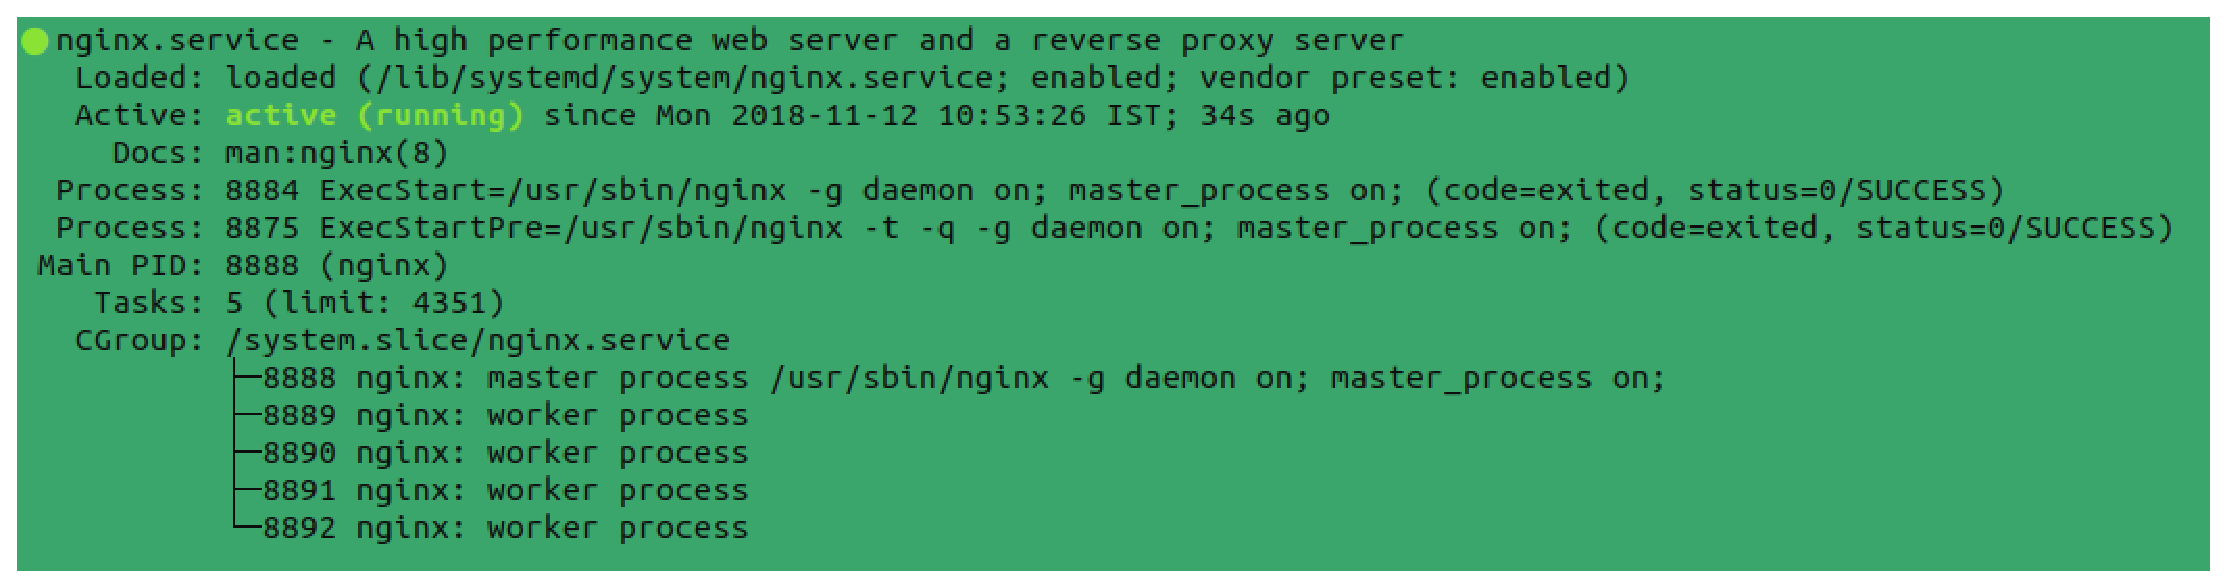
\includegraphics[scale=.5]{img1.eps}

$\bullet$ As you can see above, the service appears to have started successfully. However, the best way to test this is to actually request a page from Nginx.\\
\medskip
You can access the default Nginx landing page to confirm that the software is running properly. You can access this through your server's domain name or IP address. To find the IP address type \textit{ifconfig} on terminal.\\
\medskip
When you have your server's IP address or domain, enter it into your browser's address bar:\\
\medskip
\begin{lstlisting}[frame=single,linewidth=15cm,breaklines=true]
http://server_domain or directly write the IP address
\end{lstlisting}
\bigskip
You should see the default Nginx landing page, which should look something like this:\\
\medskip
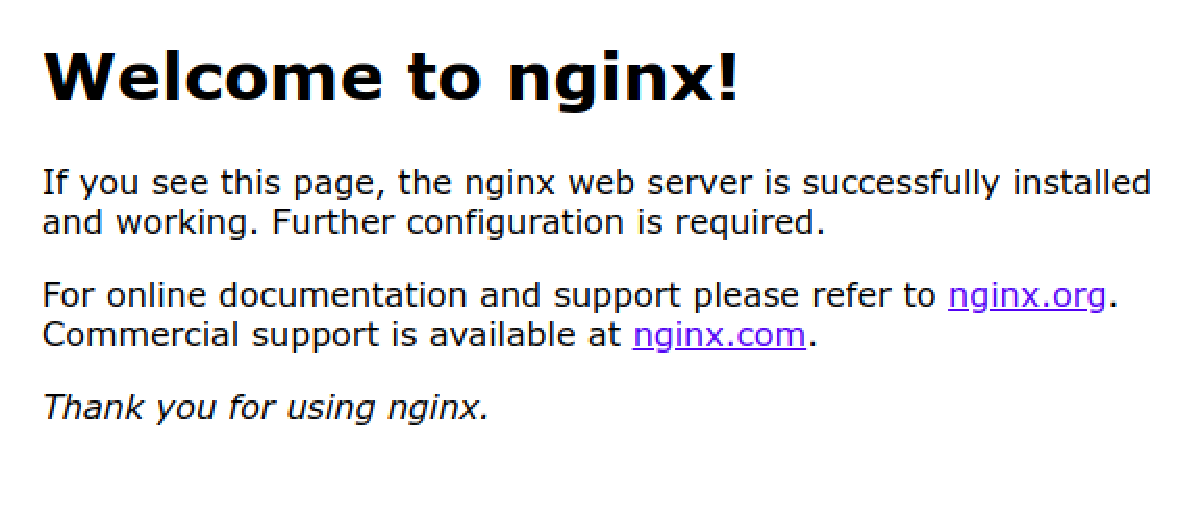
\includegraphics[scale=.4]{img2.eps}

This page is simply included with Nginx to show you that the server is running correctly.\\
\medskip
\textbf{Manage the Nginx Process:} \\
$\bullet$ Now that you have your web server up and running, we can go over some basic management commands.\\
\medskip
To stop your web server, you can type:\\
\medskip
\begin{lstlisting}[frame=single,linewidth=7cm,breaklines=true]
sudo systemctl stop nginx
\end{lstlisting}
\bigskip
\medskip
To start the web server when it is stopped, type:\\
\medskip
\begin{lstlisting}[frame=single,linewidth=10cm,breaklines=true]
sudo systemctl start nginx
\end{lstlisting}
\bigskip
\medskip
To stop and then start the service again, type:\\
\medskip
\begin{lstlisting}[frame=single,linewidth=10cm,breaklines=true]
sudo systemctl restart nginx
\end{lstlisting}
\bigskip
\medskip
By default, Nginx is configured to start automatically when the server boots. If this is not what you want, you can disable this behavior by typing: \\
\medskip
\begin{lstlisting}[frame=single,linewidth=10cm,breaklines=true]
sudo systemctl disable nginx
\end{lstlisting}
\bigskip
\medskip
To re-enable the service to start up at boot, you can type:\\
\medskip
\begin{lstlisting}[frame=single,linewidth=10cm,breaklines=true]
sudo systemctl enable nginx
\end{lstlisting}
\bigskip
\medskip
If you are simply making configuration changes, Nginx can often reload without dropping connections. To do this, this command can be used:\\
\medskip
\begin{lstlisting}[frame=single,linewidth=9cm,breaklines=true]
sudo systemctl reload nginx
\end{lstlisting}
\bigskip

\textbf{Get Familiar with Important Nginx Files and Directories:} \\
Now that you know how to manage the service itself, you should take a few minutes to familiarize yourself with a few important directories and files.\\

$\bullet$ \textbf{Content}\\
\textsf{/var/www/html:} The actual web content, which by default only consists of the default Nginx page you saw earlier, is served out of the /var/www/html directory. This can be changed by altering Nginx configuration files.\\
\bigskip
$\bullet$ \textbf{Server Configuration}\\
\medskip
\textsf{/etc/nginx:} The Nginx configuration directory. All of the Nginx configuration files reside here.\\
\medskip
\textsf{/etc/nginx/nginx.conf:} The main Nginx configuration file. This can be modified to make changes to the Nginx global configuration.\\
\medskip
\textsf{/etc/nginx/sites-available/:} The directory where per-site "server blocks" can be stored. Nginx will not use the configuration files found in this directory unless they are linked to the sites-enabled directory. Typically, all server block configuration is done in this directory, and then enabled by linking to the other directory.\\
\medskip
\textsf{/etc/nginx/sites-enabled/:} The directory where enabled per-site "server blocks" are stored. Typically, these are created by linking to configuration files found in the sites-available directory.\\
\medskip
\textsf{/etc/nginx/snippets:} This directory contains configuration fragments that can be included elsewhere in the Nginx configuration. Potentially repeatable configuration segments are good candidates for refactoring into snippets.\\
\bigskip
$\bullet$ \textbf{Server Logs:} \\
\medskip
\textsf{/var/log/nginx/access.log:}  Every request to your web server is recorded in this log file unless Nginx is configured to do otherwise.\\
\medskip
\textsf{/var/log/nginx/error.log:}  Any Nginx errors will be recorded in this log.\\
\medskip
$\bullet$ \textbf{To Add Media Files On Nginx Server} \\
To add media files on nginx server we need to do changes in configuration file. First open the default.conf using the following command:
\medskip
\begin{lstlisting}[frame=single,linewidth=15cm,breaklines=true]
sudo nano /etc/nginx/sites-available/default.conf
\end{lstlisting}
\bigskip
Now edit the file in the inside the location block write \textit{autoindex on;} as given below:
\medskip
\begin{lstlisting}[frame=single,linewidth=15cm,breaklines=true]
 location / {
                # First attempt to serve request as file, then
                # as directory, then fall back to displaying a 404.
                try_files $uri $uri/ =404;
                autoindex on;
        }

\end{lstlisting}
\bigskip
as shown in given figure:\\
\includegraphics[scale=.2]{img3.eps} \\
\bigskip
After editing the file press ctrl+x and press y then enter to modify and save the file. 
Now open terminal then go to /var/www/html page and remove the default html page using rm command login with root to remove.
Now put any file in that directory(/var/www/html). Here you can put any file inside the this directory and access it with following domain or IP address.\\
\medskip
Now open the browser and write the ip address or domain name to access the files.It should be look like this:\\
\medskip
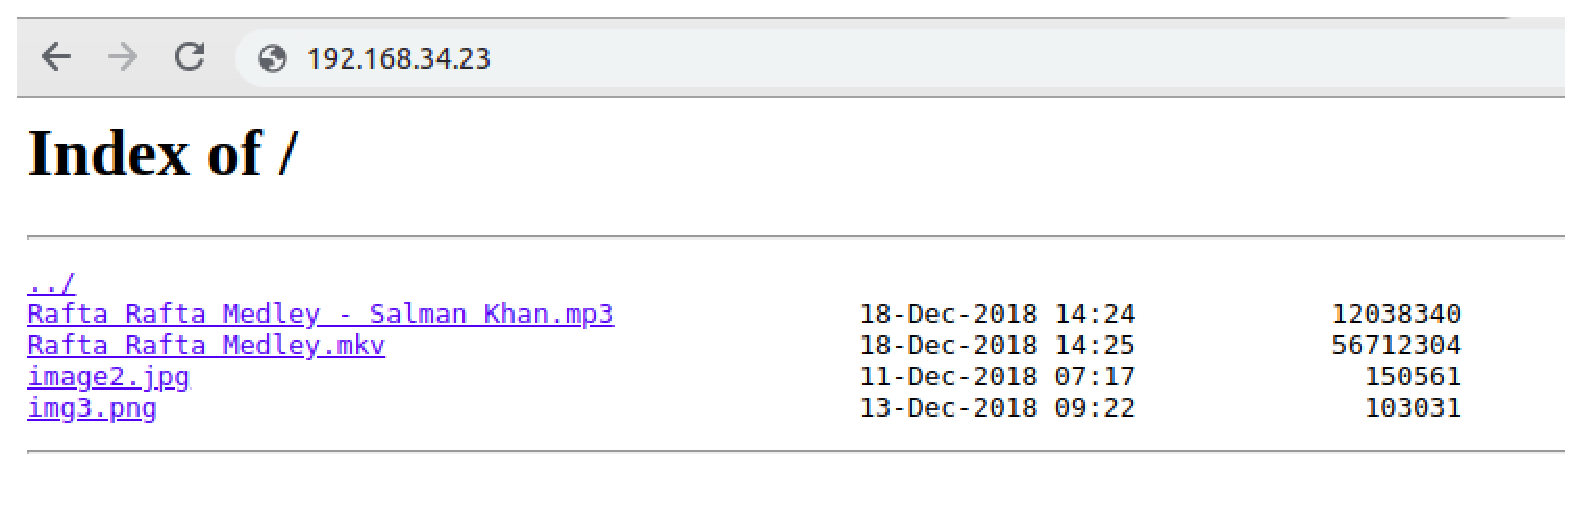
\includegraphics[scale=.5]{img7.eps} \\
\bigskip

\item {\textbf{Installing the Apache Web Server:}} \\
$\bullet$ Apache is a free, open-source HTTP server for Unix-like operating systems and Windows. It was designed to be a secure, efficient and extensible server that provides HTTP services in sync with the prevailing HTTP standards.\\
$\bullet$ \textbf{Some of the busy sites powered by Apache:}\\
PayPal, BBC.com, BBC.co.uk, SSLLABS.com, Apple.com plus lots more.\\
\medskip
To install the Apache Server, open terminal and type following command:\\
\medskip
\begin{lstlisting}[frame=single,linewidth=9cm,breaklines=true]
sudo apt-get update
sudo apt-get install apache2
\end{lstlisting}
\bigskip
\textbf{Check your Web Server:} \\
\bigskip
$\bullet$ We can check with the systemd init system to make sure the service is running by typing:\\
\bigskip
\begin{lstlisting}[frame=single,linewidth=15cm,breaklines=true]
$ sudo systemctl status apache2	  #Debian/Ubuntu 
# systemctl status httpd	  #RHEL/CentOS/Fedora 
\end{lstlisting}
\bigskip
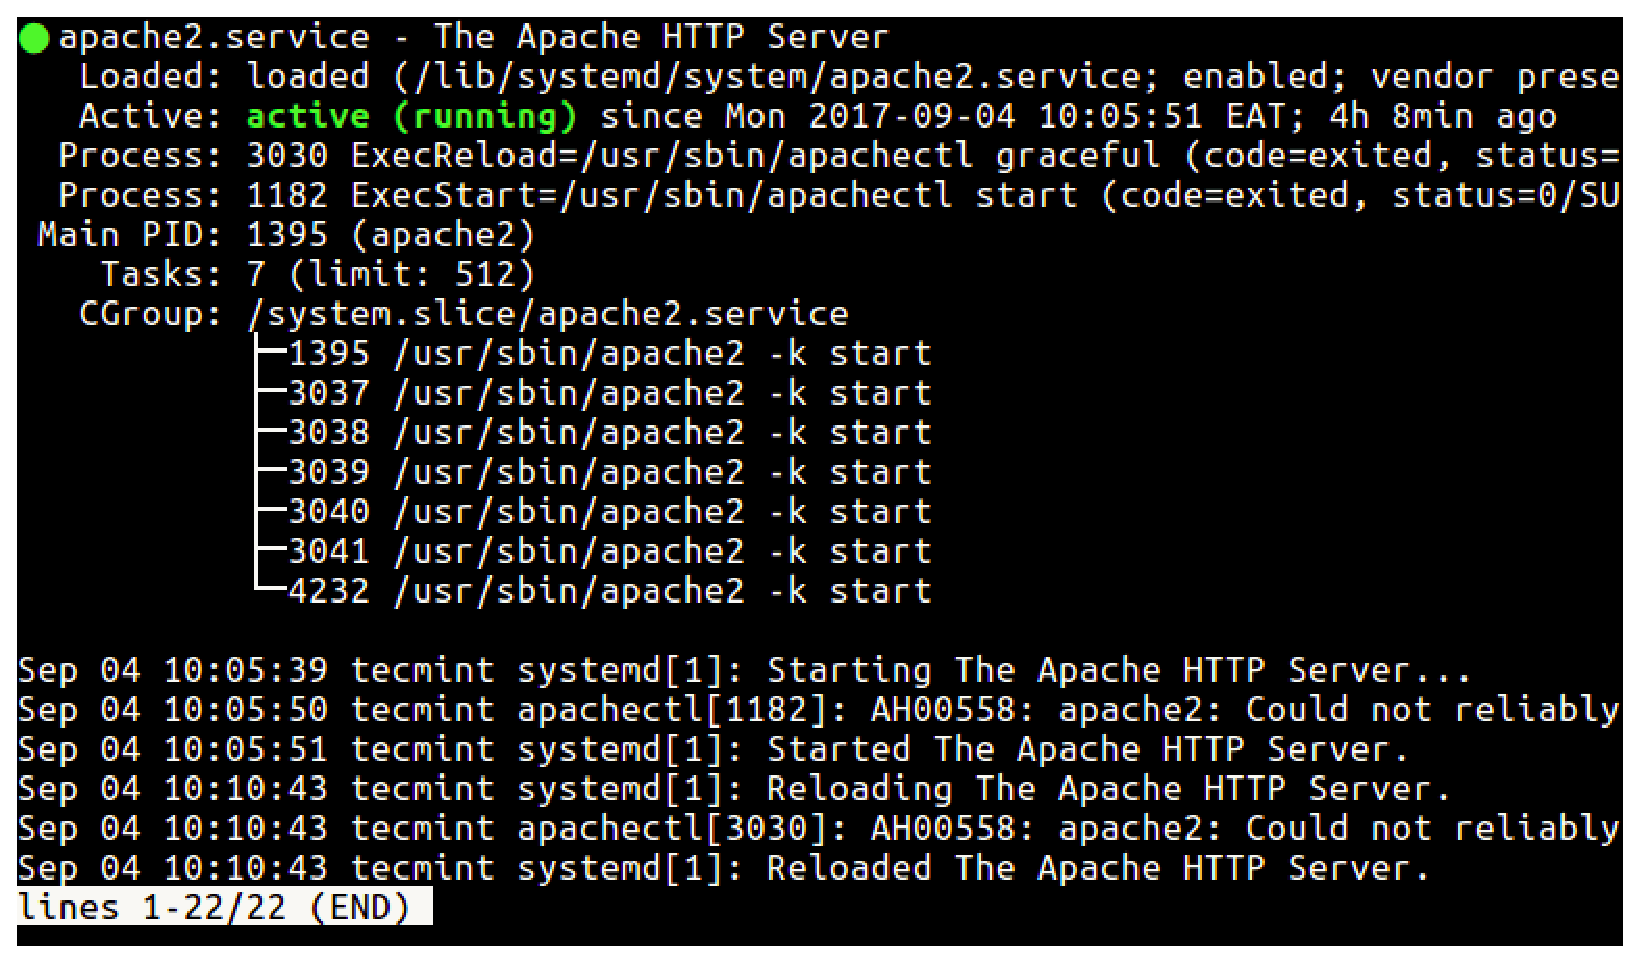
\includegraphics[scale=.3]{img6.eps}

$\bullet$ As you can see above, the service appears to have started successfully. However, the best way to test this is to actually request a page from Apache.\\
\medskip
You can access the default Apache landing page to confirm that the software is running properly. You can access this through your server's domain name or IP address. To find the IP address type \textit{ifconfig} on terminal.\\
\medskip
When you have your server's IP address or domain, enter it into your browser's address bar:\\
\medskip
\begin{lstlisting}[frame=single,linewidth=15cm,breaklines=true]
http://server_domain or directly write the IP address
\end{lstlisting}
\bigskip
You should see the default Apache landing page, which should look something like this:\\
\medskip
\includegraphics[scale=.4]{img4.png}

This page is simply included with Apache to show you that the server is running correctly.\\
\bigskip
Now open terminal then go to /var/www/html page and remove the apache default index.html page using rm command login with root to remove.
Now put any file in that directory(/var/www/html). Here you can put any file inside the this directory and access it with following domain or IP address.\\
\medskip
Now open the browser and write the ip address or domain name to access the files.\\
\bigskip

Now that you have your web server installed, you have many options for the type of content to serve and the technologies you want to use to create a richer experience.\\
\medskip
\item{\textbf{Installing the FTP server:}} \\
Open terminal and type the following command: \\
\medskip
\begin{lstlisting}[frame=single,linewidth=9cm,breaklines=true]
sudo apt-get update
sudo apt install proftpd
\end{lstlisting}
\bigskip
During installation, the window below will appear, select standalone here. if it is not appear then don’t panic, by default it will be standalone.\\
\medskip
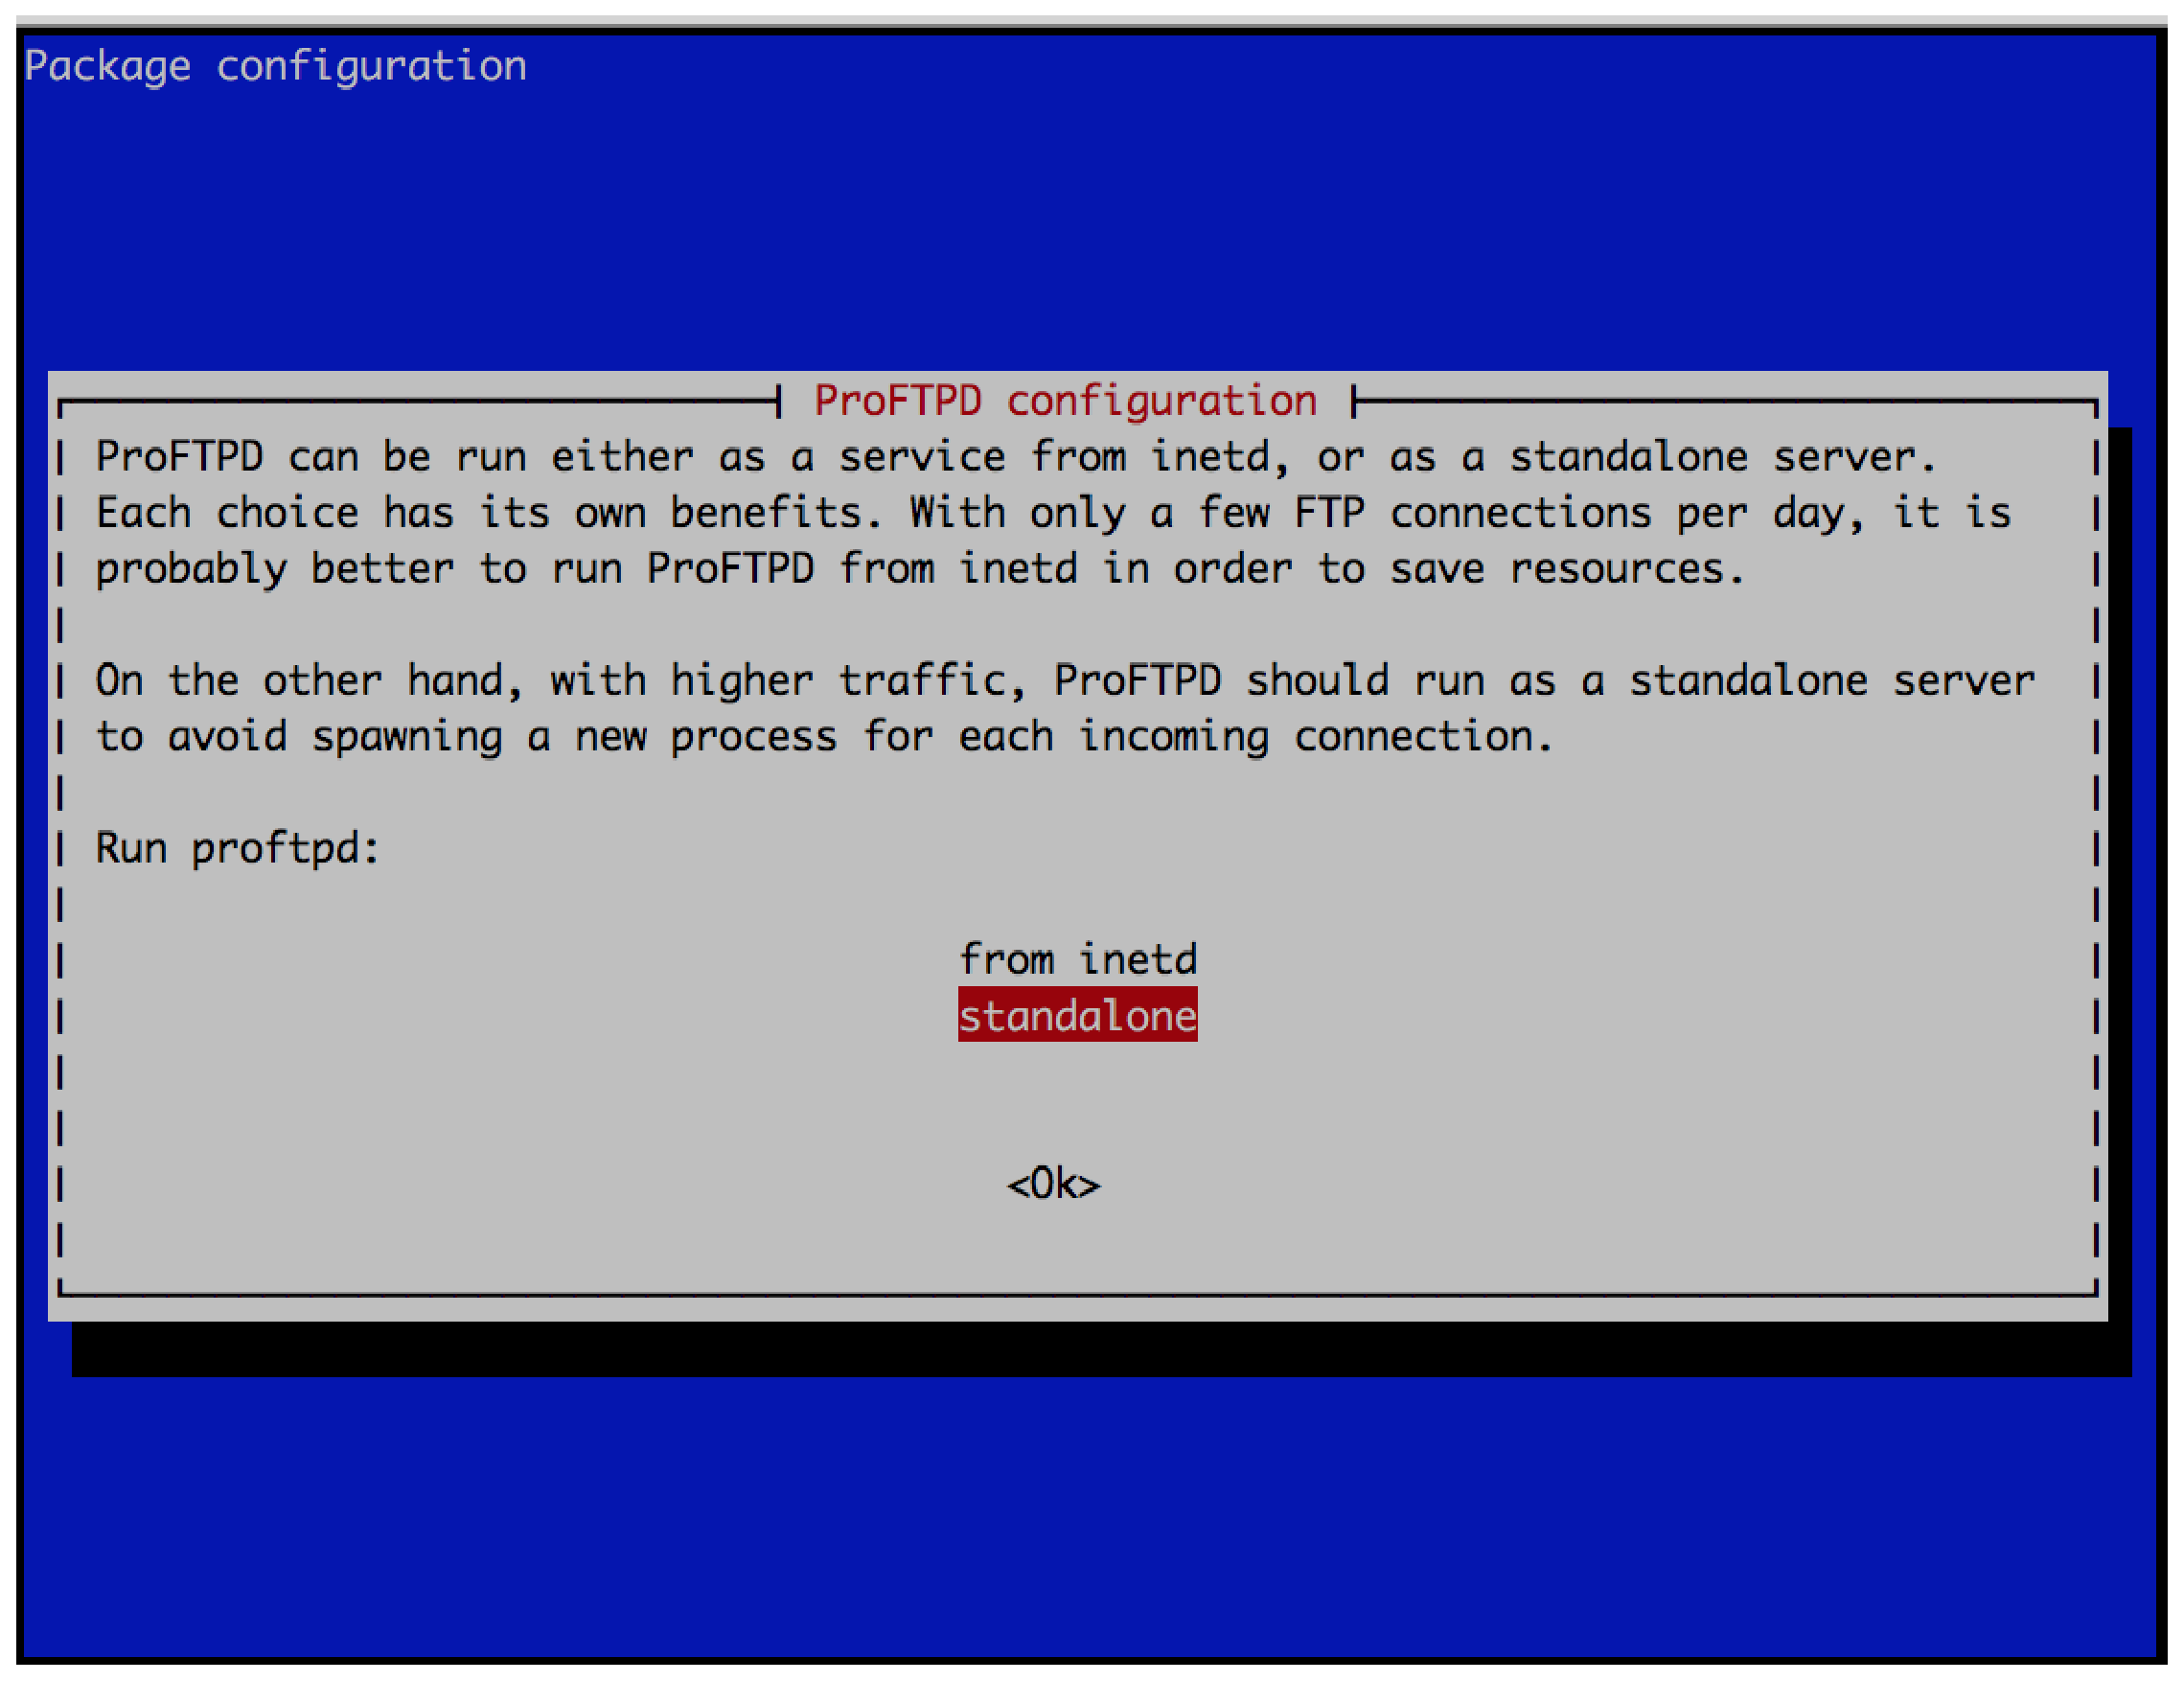
\includegraphics[scale=.2]{img8.eps} \\
\medskip
Standalone that will let the FTP server run 24/7 which allows to speed up the connection and which is convenient in case a high number of connection is expected.\\
\bigskip
$\bullet$ {\textbf{Configuring proftpd:}} \\
Type the following command to modify the the configuration file. However, there are a lot of configuration lines. We will consider the one that we consider the most important.\\
\medskip
\begin{lstlisting}[frame=single,linewidth=9cm,breaklines=true]
sudo nano /etc/proftpd/proftpd.conf
\end{lstlisting}
\bigskip
\textbf{TimeoutIdle :} which corresponds to the idle time in seconds after which a user will be automatically disconnected.By default it will be 1200. YOu can change according to you.\\
\medskip
if you want your FTP server to be public, you can allow all users to log in without a password. To do this, all the lines in the block between $<Anonymous ~ ftp> and </ Anonymous>$ must be uncommented (by removing all \# at the beginning of the lines). If it still ask user name then  use a username, "anonymous" but without a password.\\
\medskip
After you have finished configuring proftpd, you can enable the changes by running the command: \\
\begin{lstlisting}[frame=single,linewidth=9cm,breaklines=true]
sudo service proftpd reload
\end{lstlisting}
\bigskip
$\bullet${\textbf{default location:} } \\
The default location of files is /srv/ftp/  \\
\bigskip
$\bullet${\textbf{Access your FTP server}}  \\
just type ftp://ip-raspberry on the browser to access the files.
\end{enumerate}
\end{flushleft}
\begin{thebibliography}{9}
\bibitem{raspberry} 
https://www.raspberrypi.org/documentation/configuration/wireless/access-point.md
\bibitem{Nginx}
https://www.nginx.com/
\bibitem{Nginx installation and Setup }
https://www.digitalocean.com/community/tutorials/how-to-install-nginx-on-ubuntu-16-04\#step-3-check-your-web-server
\bibitem{Apache2 installation and Setup }
https://www.digitalocean.com/community/tutorials/how-to-install-linux-apache-mysql-php-lamp-stack-on-ubuntu-16-04\#step-1-install-apache-and-allow-in-firewall
\end{thebibliography}
\end{document}